\section{Results}
\label{sec:four}

Show off performance characteristics for each method using f-measure and MSE,
like in this Table~\ref{tab:regperf}.

\begin{table}[t]
  \caption{Regression performance comparison of (1) baseline, (2) linear
    regression and (3) polynomial regression of degree two as measured using the
    mean squared error on the test data set.}
  % \centering\small
  % \renewcommand{\tabcolsep}{1pt}
  \newcolumntype{C}{>{\centering\arraybackslash}X}%
  % \newcolumntype{R}{>{\raggedleft\arraybackslash}X}
  \begin{tabularx}{\linewidth}{@{\kern3pt}cCc@{\kern3pt}}
    \toprule
    \bfseries Model & \bfseries Top-$k$ Features & \bfseries MSE \\
    \midrule
    (1) & --- &  12.60835 \\
    (2) &  10 &  0.047144 \\
    (3) &  13 &  0.032151 \\
    \bottomrule
  \end{tabularx}
\label{tab:regperf}
\end{table}

\begin{table}[t]
  \caption{Classification performance comparison of (1) baseline, $k$-NN with
    (2) 1 and (3) 5 neighbors, random forest with (4) 10 and (5) 50 decision
    trees as measured using the \fmeasure{} on the test data set.}
  % \centering\small
  % \renewcommand{\tabcolsep}{1pt}
  \newcolumntype{C}{>{\centering\arraybackslash}X}%
  % \newcolumntype{R}{>{\raggedleft\arraybackslash}X}
  \begin{tabularx}{\linewidth}{@{\kern3pt}cCc@{\kern3pt}}
    \toprule
    \bfseries Model & \bfseries Top-$k$ Features & \bfseries \fmeasure{} \\
    \midrule
    (1) & --- & 0.771499 \\
    (2) &   4 & 0.805405 \\
    (3) &   4 & 0.799732 \\
    (4) &   6 & 0.812203 \\
    (5) &   6 & 0.814915 \\
    \bottomrule
  \end{tabularx}
\label{tab:clsperf}
\end{table}

\begin{figure*}[h]
\centering
\begin{minipage}{.49\textwidth}
  \centering
  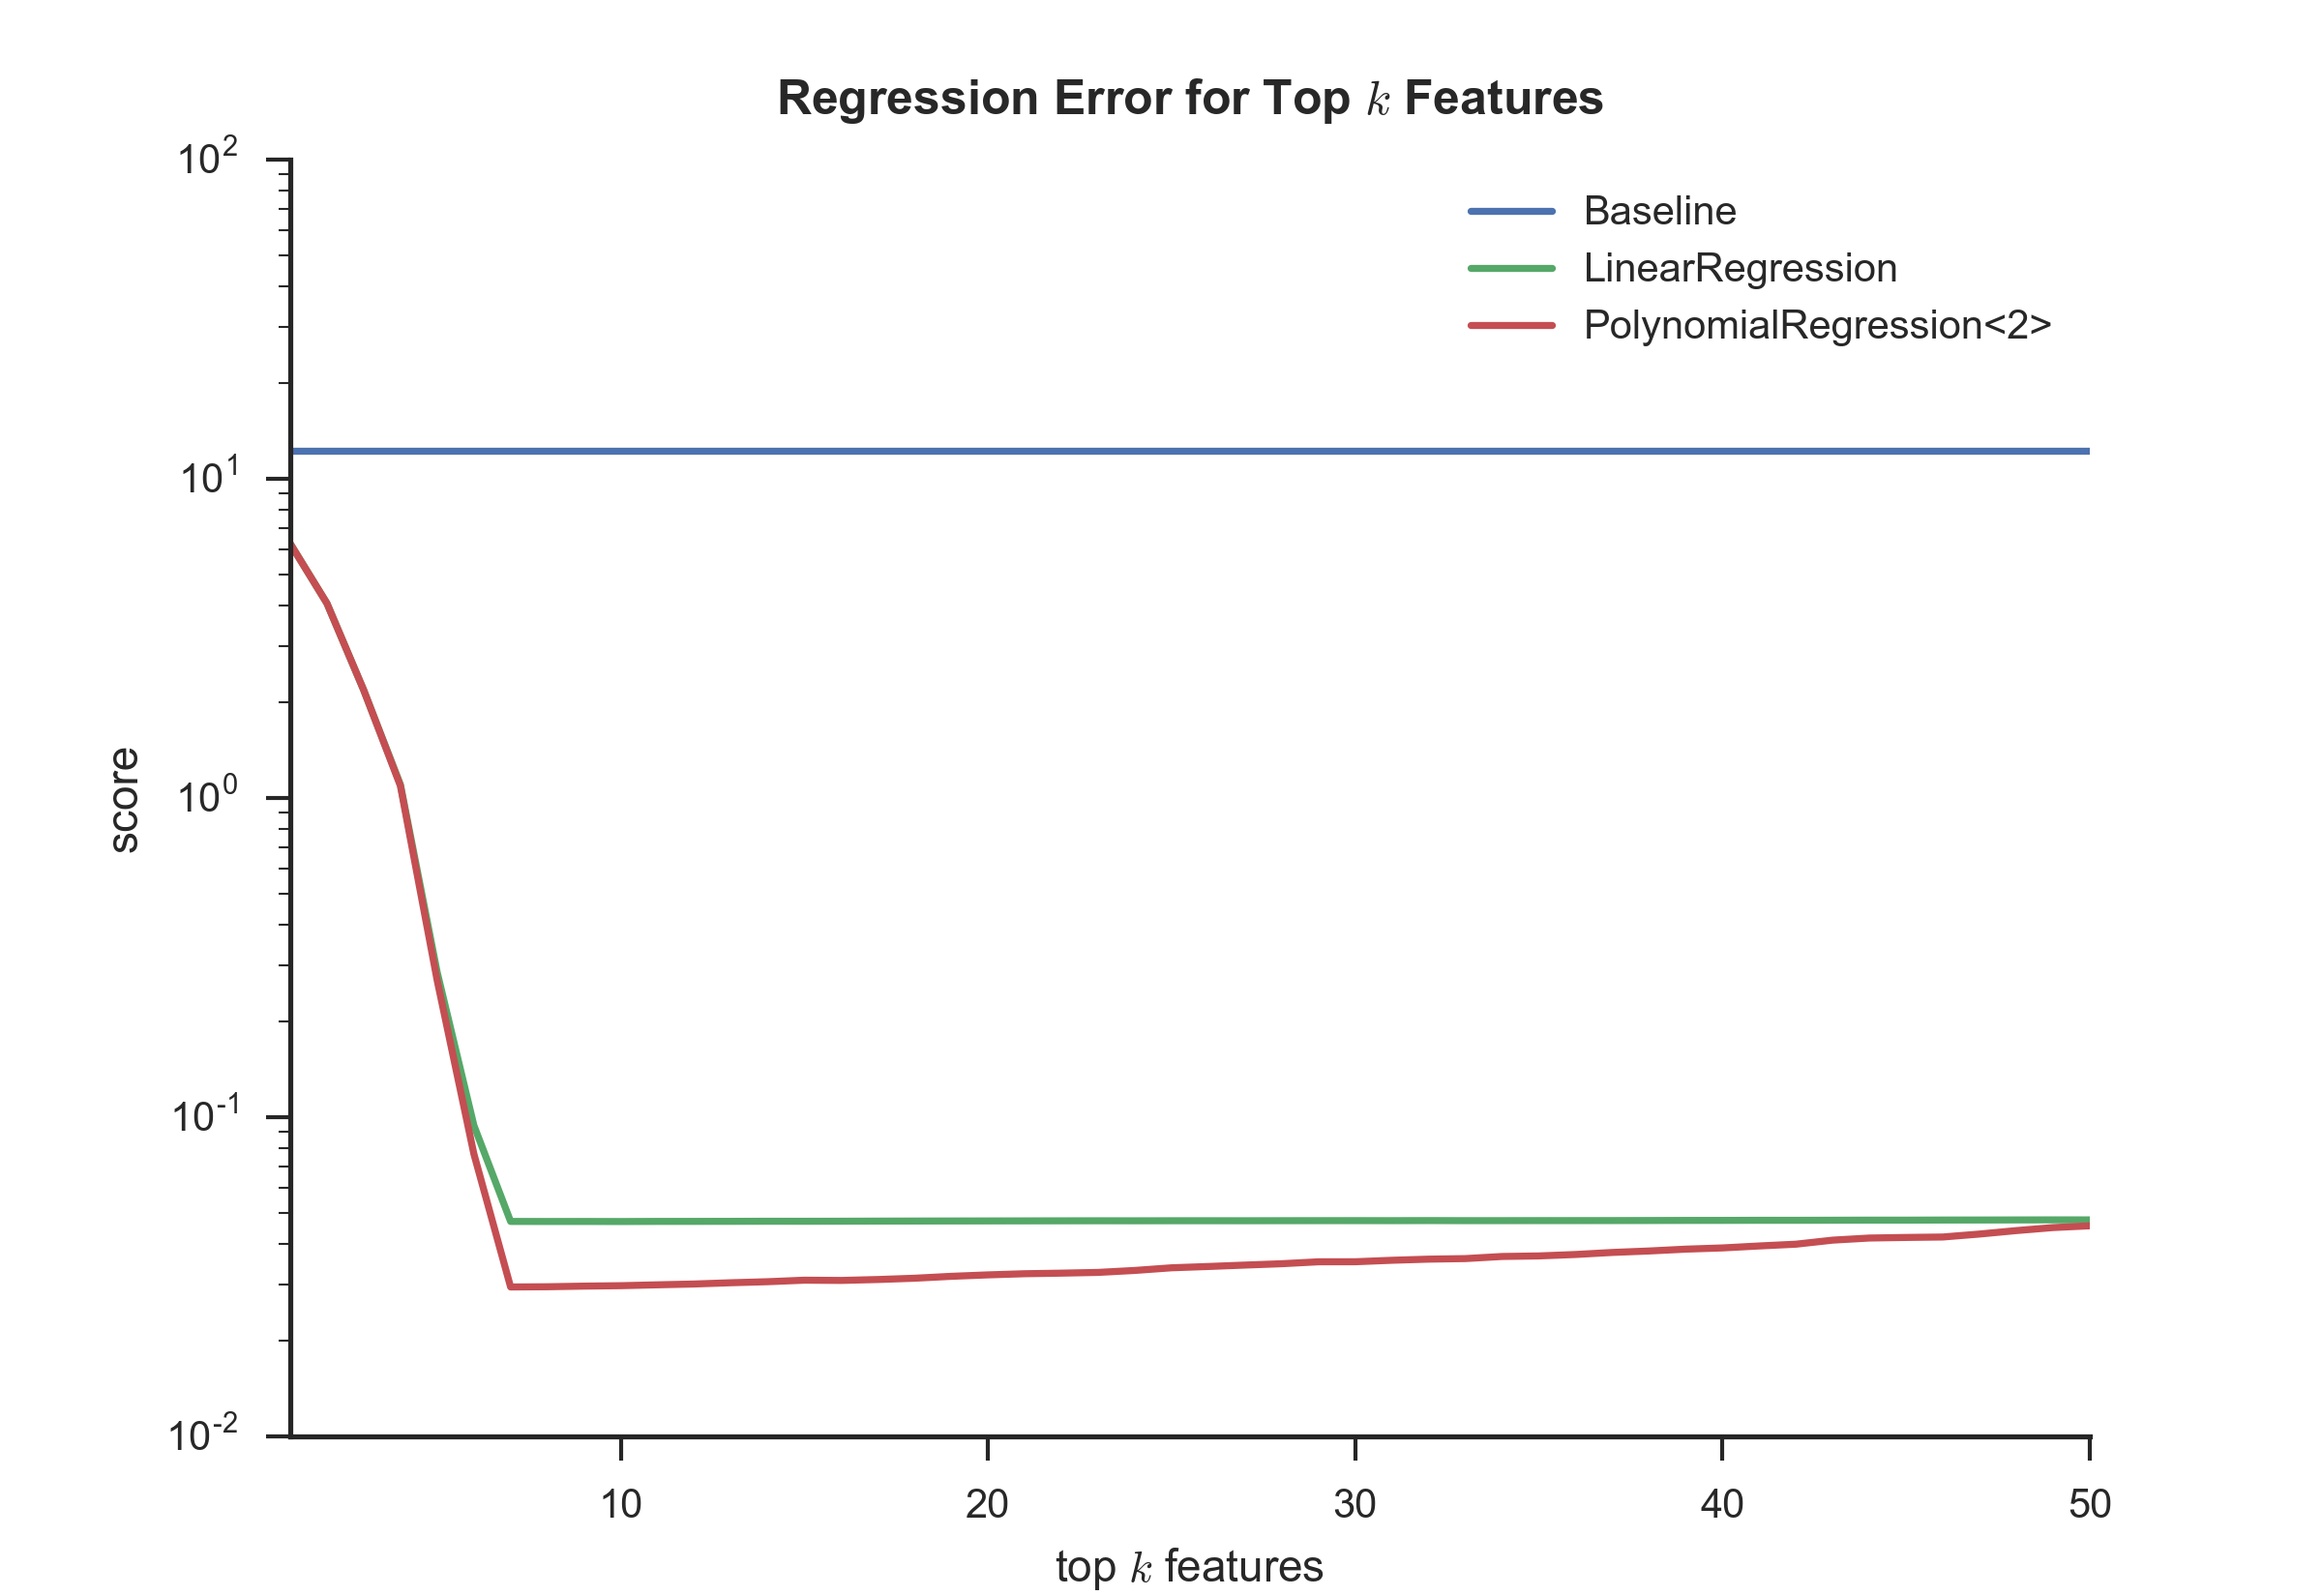
\includegraphics[width=\linewidth]{figures/reg_mse_train.png}
\end{minipage}
\begin{minipage}{.49\textwidth}
  \centering
  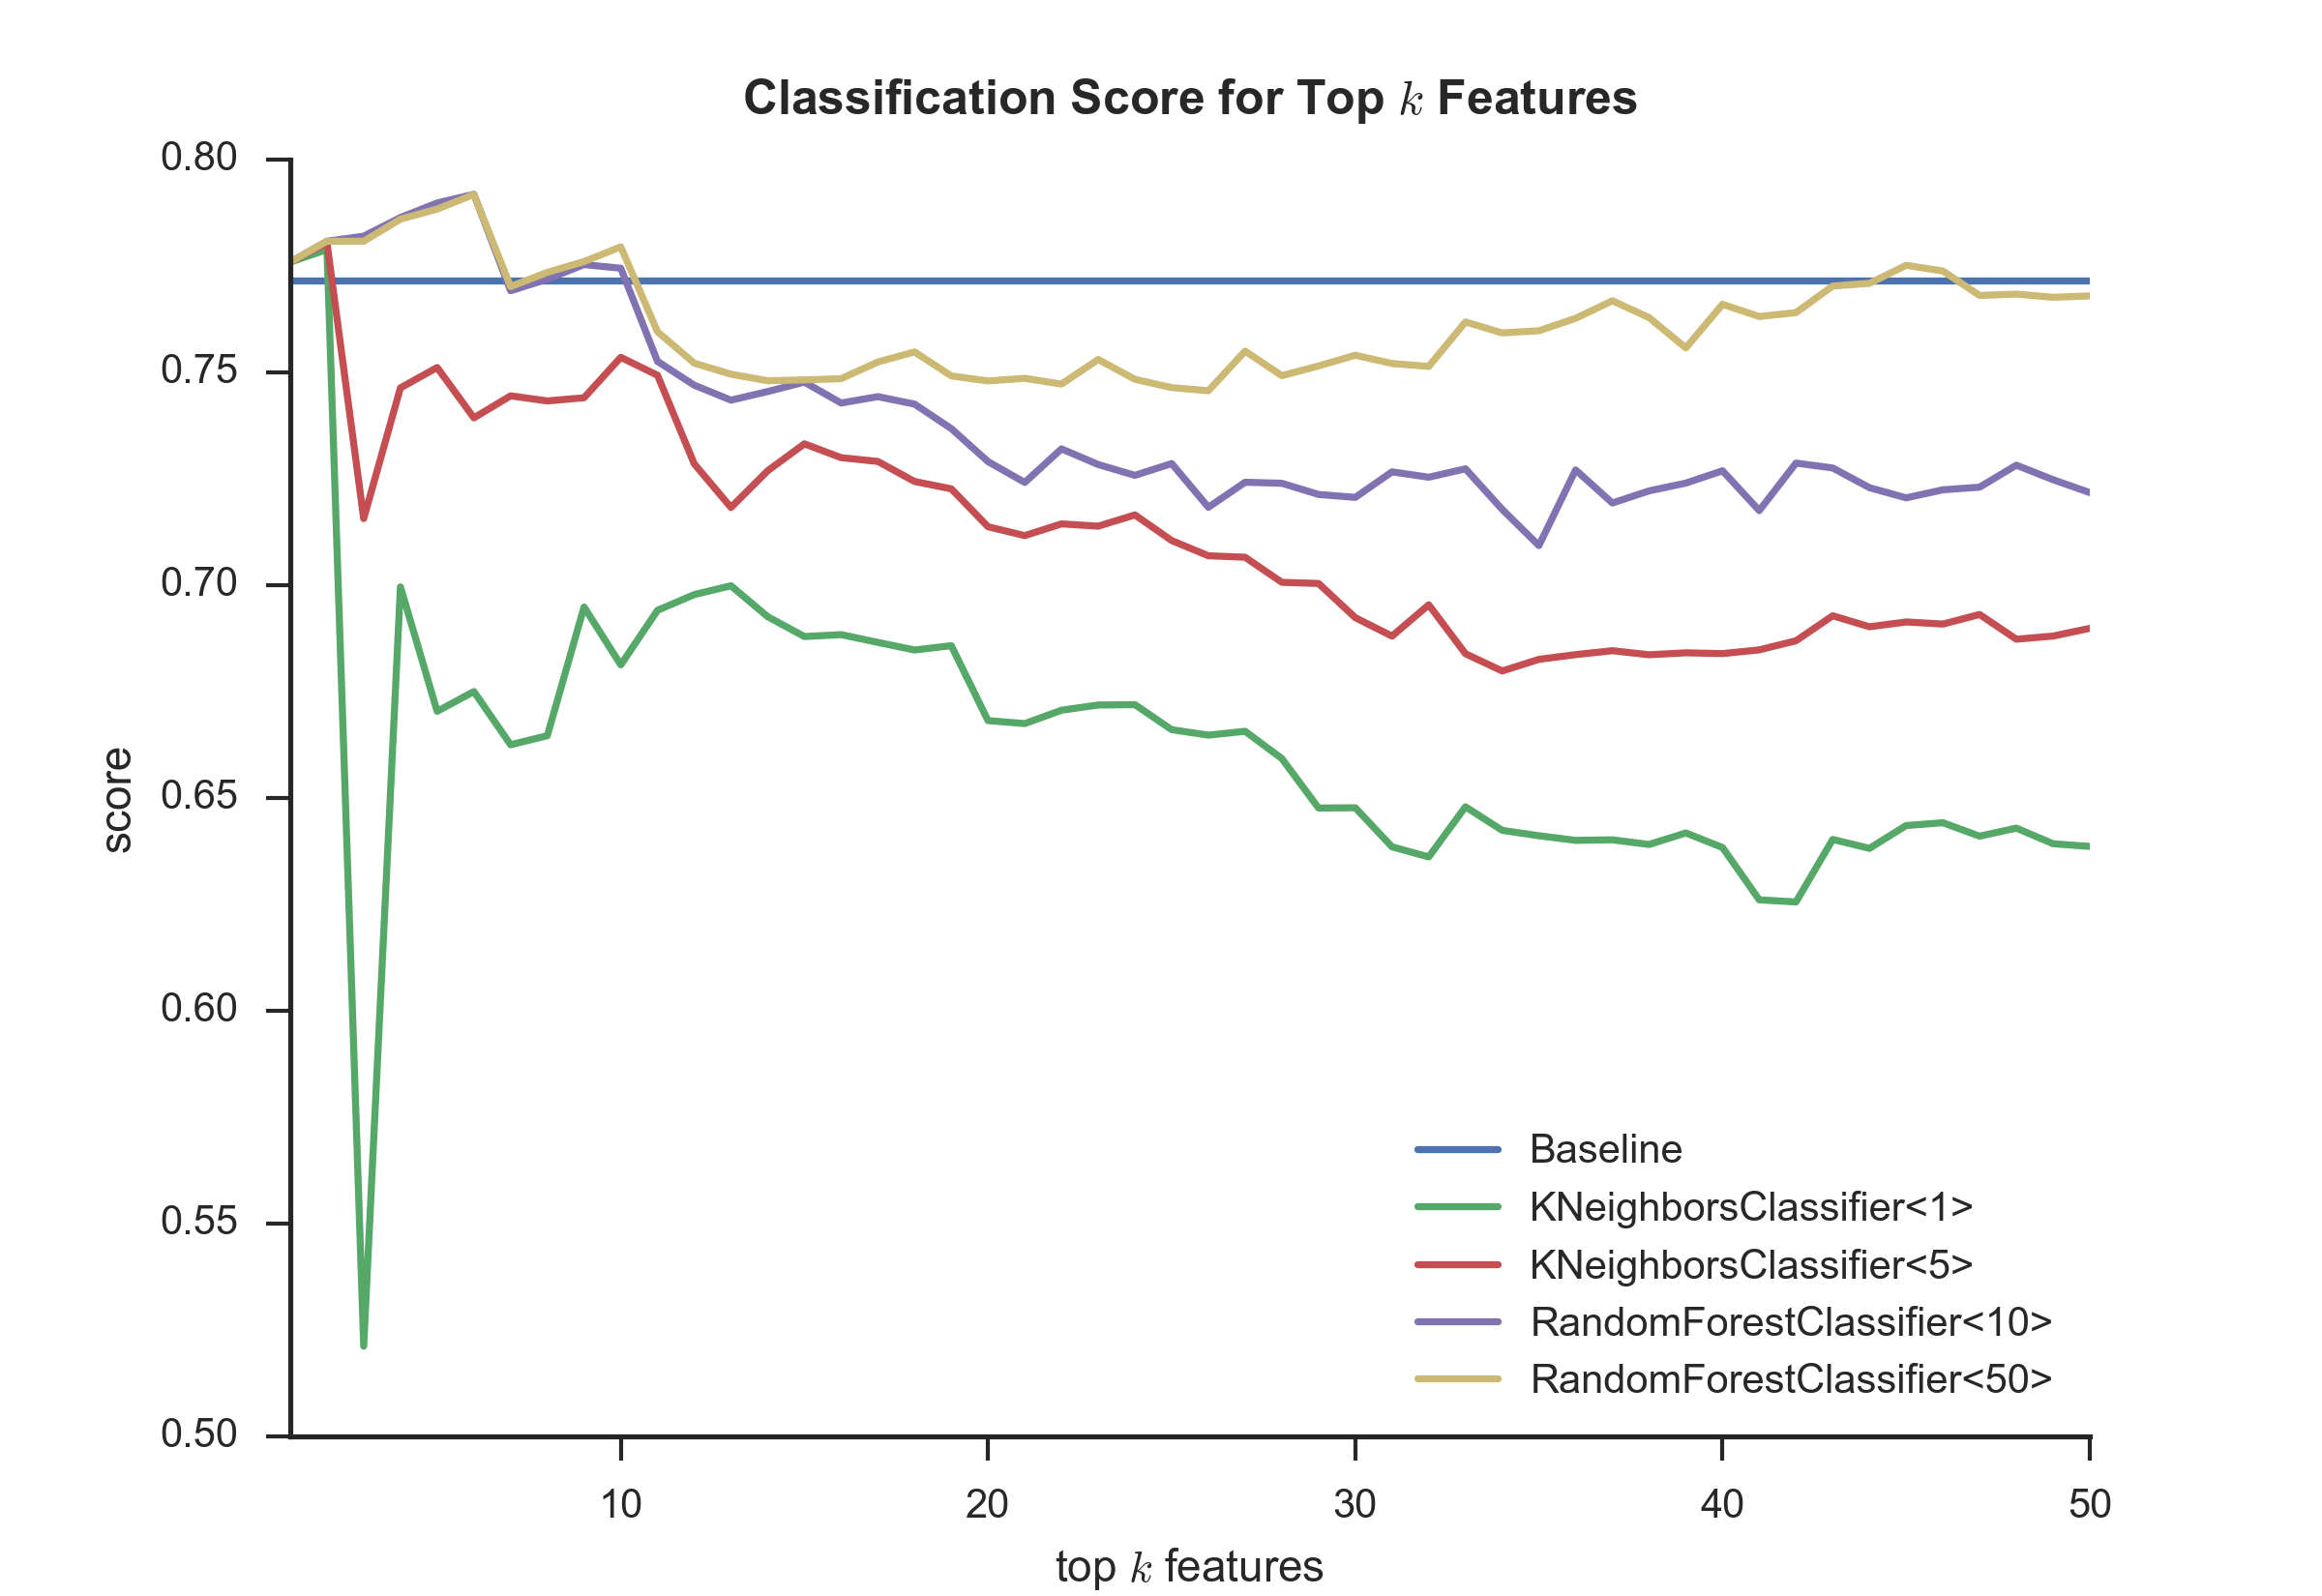
\includegraphics[width=\linewidth]{figures/cls_fscore_train.png}
\end{minipage}
\caption{Performance graphs for regression (left) and classification (right) for
  number of top-$k$ features, evaluated with MSE and \fmeasure, respectively.}
\label{fig:training}
\end{figure*}

%%% Local Variables:
%%% mode: latex
%%% TeX-master: "../main"
%%% End:
